\documentclass[a4paper]{article}
\usepackage{graphicx}

\begin{document}

\title{For Whom the Bell Tolls}

\author{Sergey Feranchuk \\{\small(self-employed; residence: Smolensk, Russia; e-mail: feranchuk@gmail.com)}}

\maketitle

\begin{flushright}
{\small \textit{to my mother}}
\end{flushright}

\section*{Abstract}

%Речь в работе идет о соотношении периодических ритмов с нерегулярными. Более узко, для микро-экосистем почвы, периодические пожары приводят к обновлению экосистем, как и намеренное регулярное освобождение от посевов, для  сельскохозяйстенных земель. Образцы почвы, и из человека - посмотрели состав микроорганизмов. Смотрели "по крупному", обзорно.

%В таком взгляде много общего, между разными сообществами микроорганизмов. То что бы можно было тут увидеть - признаки нестабильности, скрытой накопившейся нестабильности вследствии изменений режима периодичных воздействий на микро-сообщества в последние десятиления.


\section{Introduction}

Harmonic oscillator is a simplest mathematical model which can simulate periodic changes as a physical phenomenon. It is exactly solvable both in classical and in quantum physics. The simplest extension of harmonic oscillator model is to introduce a quadratic term to the linear equation of the model. 

The changes in the surrounding nature are often distinguish from a harmonic periodicity. The marginal cases of unharmonicity are a chaotic noise and an abrupt crash. Attempts to manage these extreme cases by means of ''traditional'' science are knowingly wrong, although some empirical rules do observed in these processes.

Suitable for a minimally simple approach to systematically describe in some way the possible distortions of a periodicity is the model of harmonic oscillator with an introduced perturbation, like the unharmonic oscillator model mentioned above. 

The problem in any crash is to be ready for it, and the prediction of crash is impossible. As in the cases of a phase transition, the mixing of large-scaled and local-scale factors occurs and is of importance in a transitional period. Anyway any clever decisions in a crisis time are always based on a rational reasoning even if this reasoning do not fit to a format of a ''traditional'' science which has been developed for another purposes.

As an attempt to rationally describe the risks which are accumulated in microbial communities at resent times, a wide and broad look is proposed here to a composition of some selected communities. The simple model of unharmonic oscillations can be of use to measure and clarify in some way an unharmonicity in the composition of the communities.

Recent advances in sequencing technologies lead to the ''outbreak'' in the microbiology. A wide classes and even kingdoms of poorly known living creatures become visible in the common and custom microbiological samples. The present research is focused on eukariotic part of the microbiomes for the purposes declared in it. Besides the kingdoms of animals, plants and fungi, it is presently extended to include much of another eukariotic species, mostly unicellular, hardly classified and poorly investigated. Some of them are supposed to be conservative and neutral, some are highly adaptive and predator-oriented. The group of eukariotic divisions known as SAR (''\textit{Strametopiles}'',''\textit{Alveolata}'',''\textit{Cercozoa}'') was introduced to broadly join the species with the latter of the strategies. These divisions are considered separately and other unicellular divisions with mostly first of the strategies are joined together in the analysis provided below.


\section{Methods} 


%Для минимально простого описания искажений периодичности, подойдет модель осциллятора с малым дополнением, внесенным в закон движения, так что в колебаниях такого ''не-гармонического'' осциллятора проявляются отклонения от гармонического закона - то что может являеться признаком потенциальной неустойчивости.

%В квантовом описании, уровни энергии такого осциллятора зависят от квантового числа не вполне линейно. Нарастающая периодичность соответствует положительному знаку в не-гармоничной поправке в модели осциллятора ($\hat H = p^2 + x^2 + \lambda x^4$), замедляющаяся перидичность - отрицательному знаку. 

%отклононения от равновесия, следуя представленным интерпретациям, возмоны в двух направлениях, условно обозначенных ниже А и Б:
%А - ускорение циклов и колебаний, то что грозит риском кризиса по типу ''внезапного обвала''..
%Б - замедление циклов и колебаний, где риском является ''угасание'' и ''растворение''.


%Так называемые ''распределения численности видов'', в экологии, - по сравнению их формы можно выявить особенности экосистем, хотя из моделей для описания их формы, никакая не универсальна, как это обсуждалось в [1]. В форме кривых распределения численности, в болшей или меньшей степени, применимы как модель "закона Ципфа-Парето", так и модель распределения Больцмана. Обе модели, которые в других ситуациях применимы вполне явно, выражают соотношение между линейным возрастанием ''энергии'' системы, от уровня к уровню, и экспоненциальным убыванием ''заселенности'' уровней; в распределении Ципфа-Парето ''энергия'' вводится неявно и выражается по логарифмическому закону. 

%Используя формулу для расчета уровней энергии, предложенную в [2], через поправки к модели Ципфа-Парето и модели Больцмана на рис. 1 показано, как отклонения от периодичности проявлялись бы в кривых распределения видов.

%были использованы, выборочно, эксперименты по определению генетического материалу микробных сообществ, сделанные разными учеными, в разное время и по разным причинам. Данные для обработки были скачаны из репозиториев, где они были депонированы теми, кто ставил эти эксперименты, 


\section{Results} 


%Кривые распределения численности для разных групп, по всем образцам совместно, показаны на рис. 2, и то что при этом интересует - как форма кривой соотносится с потенциальной неустойчивостью экосистемы. 
%Сравнение ''царств'' по кривым распределения численности



%Соотношение ''царств'' организмов, по образцам и по годам}

%дрожей много - частично от искажений внесенных неполнотой референсного списка организмов.

%по годам, группа, называемая SAR, ''перевешивает'' группы, малоизученные и, по предположениям, консервативные и нейтральные.

%Сводя вопрос сравнения численности видов к сравнению неустойчивости групп при сменах времен года, месяцев, дней и ночей, сменах дождей и яснй погоды, сменах полноводных паводков на маловодные при разливах рек - то что и определяет избыток питания в экологических нишах и под-группах, и ''заселенность'' в этих нишах - признаки искажения такой периодичности, индуцируимые через обратную связь, были бы признаком неусточивости.

%Не говоря о разнообразных группах одноклеточных организмов, про которые мало известно, для трех царст живого направления их отклонения, по диаграммам численности, показны ниже:


\section{Discussion}

%Само событие кризиса в этой модели не описывается и не предсказывается. Эмпирически, колебания с нарастающим периодом - это признак риска кризиса [3]. В рамках самой модели квантового ангармонического осциллятора, ''сбой'' его движения возможен при отрицательном $\lambda$, через тоннельный переход в один из двух сегментов с отрицательной энергией за пределами области колебаний.

%\subsection*{Паразитические и патогенные виды - индикатор неусточивосчти?}

%На рисунке выделены красным группы, включающие паразитические организмы, потенциально вызывающие хронические трудно излечимые расстройства здоровья. Это, в образцах 1,6 - \textit{Nematoda}, в образце 4 - \textit{Platyhelmintes}, паразитические черви; в образцах 1,2, как следы - \textit{Microsporidia}, паразитические организмы, выживающие внутри клеток хозяина, и многоклеточные подобно грибам; в образце 1 - \textit{Apicomplexa}, в образце 6 - \textit{Haplosporida} и следы \textit{Cnidaria} - микроорганизмы, отнесенные к \textit{Alveolata}, для которых характерно многообразие паразитических циклов,



%''прорыв'' в микробиологии позволил увидеть больше в том что относися к микроорганизмам, акценты в описаниии причин и следствий привычных явлений в этом свете другие. в микробных сообществах есть общее, прагматически, микроорганизмы с земли, микроорганизмы с растений и животных переносятся легко и адаптируются быстрее чем ''хозяева''. что касается ''пахотного цикла'', эффект от его прекращения и сокращения, сказался бы на том общем, что есть во всех вышеупомянутых типах сообществ. долгосрочное накопление напряжения такого рода, как ожидается по постановке вопроса, как и любое накопление напряжения, имеет следствием риск ''взрыва'', ''обвала'', крупномасштабного кризиса.  



\section*{Conclusions}


%В арсенале науки нет инструметов, чтобы с достоверностью обнаржить и проанализировать ход событий в переходный к кризисному период. Теория фракталов - один из методов, который применим к таким явлениям, как эмпирическое описание с заведомо мало-достоверным результатом.  Вопрос заведомо остается открытым и любые другие рациональные методы его исследовать приемлем, соразмерно с осмысленнстью полученных результатов.


\section{References}

\begin{enumerate}

\item Feranchuk, S., Belkova, N., et al., Evaluating the use of diversity indices to distinguish between microbial communities with different traits. Res. Microbiol., 2018

\item Feranchuk, I., Komarov, L., et al., Operator method in the problem of quantum unharmonic oscillator, Annals of Phys., 1995 

\item Nottale, L., Scale relativity and fractal space-time: theory and applications, arxiv.org, 2008

\end{enumerate}

\newpage
\section*{Figure 1}

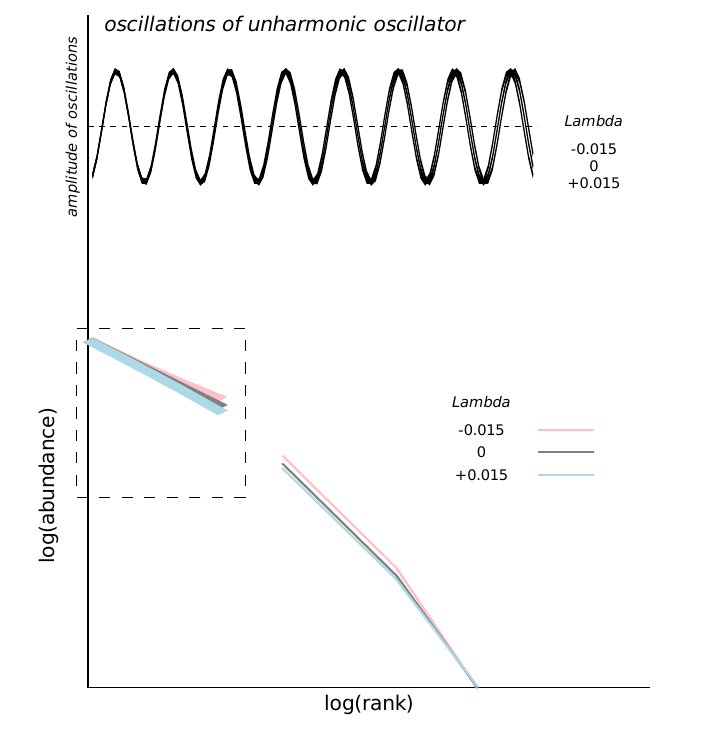
\includegraphics[width=0.7\textwidth]{rankabundance_unharmonic.jpg}

%\textit{смещение частоты колебаний и смещение модельных распределений численности, в модели Ципфа-Парето (обведено рамкой) и модели Больцмана, при разных знаках коэффициента $\lambda$ в ан-гармоническом осцилляторе}

\newpage
\section*{Figure 2} 

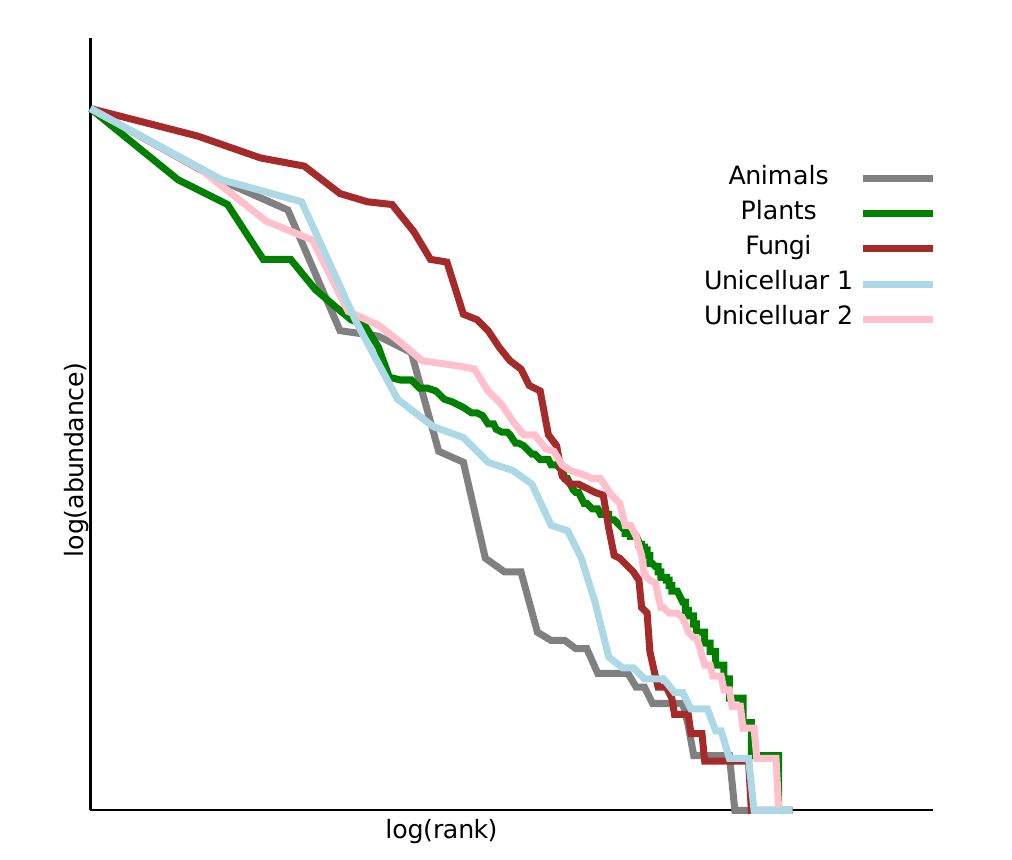
\includegraphics[width=0.7\textwidth]{rankabundance.jpg}

\textit{Кривые распределения численности, по группам организмов}; 

\vskip 10pt
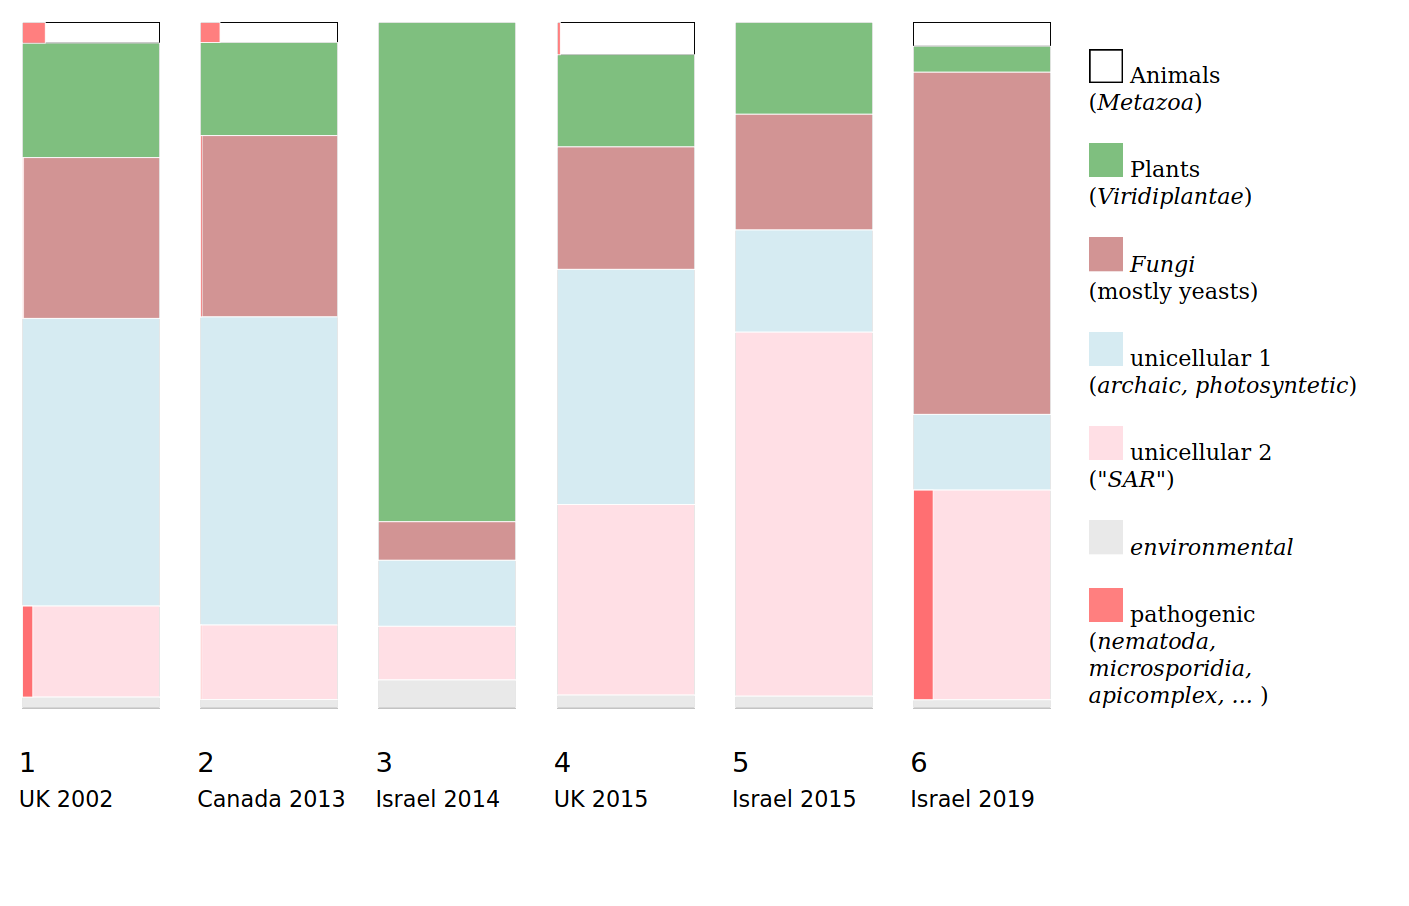
\includegraphics[width=0.99\textwidth]{tilechart.jpg}
%\textit{Соотношение состава групп организмов, по образцам - колонки соответстуют образцам}

\vskip 15pt

\newpage
\section*{Table 1} 

\begin{tabular}{lllllllll}
\hline
&Sample ID&Bases&Reads&Location&Date&18S RRNAs\\
\hline
1&ERR981203&5.3G&10M&51.83N 0.21E&2002.06.23&1517(*)\\
2&SRR6030929&2.4G&6.1M&42.98N 81.24W&2013&125002(*)\\
3&ERR588716&8.2M&159K&Israel&2014 or earlier&848\\
4&ERR970400&4.2G&13M&51.61N 3.95E&2015.01.01&18747 (*)\\
5&SRR7642476&77M&128K&30.78N 34.76E&2015.08.20&4231\\
6&SRR12806764&48M&97K&31.86N 34.72E&2019.02.25&116666\\
\hline
\end{tabular}


\newpage
\section*{Table 2} 

\begin{tabular}{ll}
\hline
Animals&\textit{Mollusca,Arthopoda}\\
Plants&\textit{Chlorophyta,Streptophyta}\\
Fungi&95\% - 100\% \textit{Saccharomycotina} (yeast)\\
Unicellular 1&\textit{Euglenozoa,Rhodophyta,Haptophyta,Glaucophyta,Cryptophyta}\\
Unicellular 2&\textit{Cercozoa,Strametopiles,Alveolata,Acanthamoeba}\\
\hline
\end{tabular}


\newpage
\section*{Table 3} 

%\textit{Количество аннотированных фрагментов рРНК по группам в каждом из образцов}

\vskip 5pt

\begin{tabular}{lllllll}
\hline
Taxonomy(*) &1&2&3&4&5&6\\
\hline
Acanthamoebidae Acanthamoeba&2&4& &1& &\\
Alveolata Apicomplexa&12&&&14& &\\
Alveolata Ciliophora&&&&2&9&1\\
Alveolata Haplosporida&&4&&&&5406\\
Cercozoa Cercomonadida&&2&&&&\\
Cercozoa Chlorarachniophyceae&4307&197&5&108&876&14637\\
Cryptophyta Cryptomonadaceae&91&&&9&389&382\\
Cryptophyta Teleaulax&&2&&&&\\
Diplomonadida Hexamitidae&19&5&&2&&\\
environmental samples&357&50&35&25&1206&1490\\
Euglenozoa Euglenida&407&84&&46&&1\\
Euglenozoa Kinetoplastida&2072&785&4&270&1206&5343\\
Fungi Ascomycota&3343&1044&&347&11860&60992\\
Fungi Basidiomycota&&&48&3&4&\\
Fungi Chytridiomycota&&&&1&&\\
Fungi Microsporidia&1&12&&3&2&12\\
Fungi Zygomycota&5&8&&&1&\\
Glaucocystophyceae Glaucocystales&77&56&&12&2890&5020\\
Glaucocystophyceae Gloeochaetales&244&8&8&9&5042&1845\\
Granuloreticulosea Foraminifera&3&&&&&\\
Haptophyceae Isochrysidales&317&103&11&24&33&19\\
Haptophyceae unclassified Haptophyceae&17&2&&1&32&24\\
Metazoa Acanthocephala&&&&&&1\\
Metazoa Arthropoda&382&12&&13&2424&627\\
Metazoa Chordata&&2&&5&&\\
Metazoa Cnidaria&&&&&&6\\
Metazoa Mollusca&475&91&&22&8907&3641\\
Metazoa Myxozoa&&&&8&&2\\
Metazoa Nematoda&&15&&&&38\\
Metazoa Platyhelminthes&26&&&&&13\\
Metazoa Porifera&&&&&6&\\
Parabasalidea Trichomonadida&2&&&1&&\\
Rhodophyta Bangiophyceae&2962&541&43&175&714&801\\
Rhodophyta Florideophyceae&232&227&16&88&148&110\\
stramenopiles Bacillariophyta&125&47&3&10&3091&312\\
stramenopiles Chrysophyceae&41&10&1&1&3&3\\
stramenopiles Olisthodiscus&379&29&&17&28&78\\
stramenopiles Oomycetes&&2&&&&\\
stramenopiles Phaeophyceae&33&6&&&1&\\
stramenopiles Placididea&303&136&57&48&33139&17046\\
Viridiplantae Chlorophyta&1636&401&478&139&1563&2569\\
Viridiplantae Streptophyta&876&315&137&113&7886&4583\\
\hline
\end{tabular}

%{\small(*) Таксономия согласно версии EBI, 2-й и 3-й уровни.}


\section*{Supplement A} 

Unharmonic oscillator

\textit{classical system:}\\
\texttt{\tiny{ awk '\{ lambda=\$1; x = 1; v = 0; dt = 0.01; s = ''''; for ( i = 1; i < 5000; i++ ) \{ x = x + v * dt; v = v - x * ( 1 + lambda * x * x ) * dt; if ( i \% 50 == 0 ) \{ s = s '' '' ( i * dt ) '','' x; \}; \}; print s \}' }} \\

\textit{C code:}\\
\texttt{\tiny{ void solve\_cubic( double h, double g, double *e1 ) \{ }} \\
\texttt{\tiny{ double d = atan2( sqrt( pow( h, 3 ) - g * g ), -g ) / 3.; }}\\
\texttt{\tiny{ double c = sqrt( h ) * cos( c ); *e1 = 2 * c; \} }} \\
\texttt{\tiny{ int main( int argc, char **argv ) \{ }} \\
\texttt{\tiny{ double lambda = atof( argv[1] ); double nmax = atoi( argv[2] ); double omega\_n; int n; }} \\
\texttt{\tiny{ for ( n = 0; n < nmax; n++ ) \{ solve\_cubic( 1. / 3., -3. * lambda * ( 1. + 2. * n + 2. * n * n ) / ( 1. + 2. * n ), \&omega\_n ); }} \\
\texttt{\tiny{ printf( ''\%.2f '', ( 1. / 4. ) * ( 3. * omega\_n + 1. / omega\_n )* ( n + 1. / 2 ) ); \} \} }} \\


Reference database\\
\texttt{\tiny{ cat ssu\_jan03.tsv | bash -c 'while read line; do if [ ''\$\{line:0:4\}'' == "tax," ]; then if [ ''\$\{line:5:5\}'' == ''Eukar'' ]; then if [''\$f'' == ''2'' ]; then echo ''\$i" ''\$\{line:5\}; i=`echo \$i + 1 | bc`; f=''1''; fi;fi;  else if [ ''\$f'' == ''1'' ]; then if [ ''\$\{line:5\}'' != '''' ]; then echo \$\{line:5\}; f=''2''; fi; fi; fi; done; ' | awk '\{ if ( \$2 == ''Eukaryota;'' || ( p == ''Eukaryota;'' \&\& length( \$0 ) > 100 ) ) \{ print \$0 \}; p = \$2 \}' | awk '\{ if ( p != \$2 ) \{ print \$0 \}; p = \$2 \} ' >rrna\_euk.fa }} \\
\texttt{\tiny{ cat \$sample | awk '\{ print substr( \$1, 1, length( \$1 ) - 1 ) \}' | bash -c 's='''';c=0;while read line; do if [ ''\$line'' != ''\$s'' ]; then if [ ''\$s'' != '''' ]; then echo ''\''\$s\'' : \$c,''; fi; s=\$line; c=1; else c=`echo ''\$c+1'' | bc`; fi; done; }} \\
\texttt{\tiny{ sort \$sample |  bash -c 's='''';c=0;while read line; do if [ ''\$line'' != ''\$s'' ]; then if [ ''\$s'' != '''' ]; then echo ''\$s \$c''; fi; s=\$line; c=1; else c=`echo ''\$c+1'' | bc`; fi; done;' | awk '\{ print \$3 '' '' \$(NF-1) '' '' \$NF \}' | sort - | bash -c 's='''';b='''';c=0;while read line; do if [ ''\$\{line:0:5\}'' != ''\$\{s:0:5\}'' ]; then h=`echo \$s |awk '''''''\{print \$1\}'''''''`; echo ''\$h \$b''; c=0; s=\$\{line\}; else n=`echo \$line | awk '''''''\{print \$NF\}'''''''`; if [ \$n -gt \$c ]; then c=\$n; b=`echo \$line | awk '''''''\{ print \$(NF-1) \}'''''''`; fi; fi; done; h=`echo \$s |awk '''''''\{print \$1\}'''''''`; echo ''\$h \$b''' }} \\

Annotation of samples\\
\texttt{\tiny{head -n 4000000 \$sample.fastq >t0.fastq}} \\
\texttt{\tiny{sortmerna --ref ssu.fa,ssu.idx --reads t0.fastq --aligned t1 --sam}} \\
\texttt{\tiny{cat t1.sam | awk '{ print ''>'' \$1 ''\\n'' \$10 }' > t2.fa}} \\
\texttt{\tiny{blastn -db ssu.db -query t2.fa -evalue 1e-2 -task blastn -max\_target\_seqs 1 -out t3.tsv -outfmt ''6 sallseqid'' out=test-\${sample}}} \\
\texttt{\tiny{mv \${out}.tsv t3.tsv }} \\
\texttt{\tiny{cat t3.tsv | while read line; do t=`grep ''>\$line '' ssu.fa`; echo \${t:1} >>\$out.txt; done; }} \\
\texttt{\tiny{cat \$out.txt | awk '{ gsub(/[0-9]/,''''); gsub( ''; '', '','' ); print }' | sort >\${out}.csv }} \\
\texttt{\tiny{cat \$out.csv | awk -F '','' '{ print \$2 '' '' \$3 }' | bash -c 's='''';c=0;while read line; do if [ ''\$line'' != ''\$s'' ]; then if [ ''\$c'' != ''0'' ]; then echo ''  \''\$s\'' : \$c,''; fi; s=\$line; c=1; else c=`echo ''\$c+1'' | bc`; fi; done; echo ''  \''\$s\'' : \$c'';'; }} \\

Rank-abundance charts\\
e.g, SAR:\\
\texttt{\tiny{grep -E 'Cercozoa|strametopiles|Alveolata|Acanthamoeba' test*.txt | sort | awk '\{ print \$1 \}' |  bash -c 's='''';c=0;while read line; do if [ ''\$line'' != ''\$s'' ]; then if [ ''\$s'' != '''' ]; then echo \$c; fi; s=\$line; c=1; else c=`echo ''\$c+1'' | bc`; fi; done; echo \$c' | sort -g | awk '\{ s = \$0 '' '' s \} END \{ print s \}' | awk '\{ s = ''''; for ( i=1; i <= NF; i++ ) \{ s = s '' '' log(i)/log(NF) '','' log(\$i)/log(\$1) \}; print s \}' }}\\

 
Rna-seq

rank-abundance

for ft in FAL MAL FCR MCR; do for cn in 28 29 30; do cat RNAseq\_WT\$ft.csv | awk -F "," -v cn=\$cn -v i=0 '\{ if ( \$cn > 0 \&\& i > 0 ) print \$cn; i = i + 1 \}' | sort -g -r | awk -v sname="'"\$ft\$cn"'" 'BEGIN \{ print sname ":["; s = ""; i = 0 \} \{ i = i + 1; if ( ( i \% 20 ) == 0 ) \{ print s ","; s = \$1 \} else \{ if ( i > 1 ) \{ s = s "," \$1; \} else \{ s = \$1 \} \}; \} END \{ print s "]," \}' >>rnaseq\_distributions.txt; done; done;

fractal dimension:

{\texttt \small
awkcmd='\{ n1 = abs( \$1 - \$2 ) + abs( \$2 - \$3 ) + abs ( \$3 - \$4 ) + abs(  \$4 - \$5 ) + abs( \$5 - \$6 ); n2 = 0.5 * ( abs(  \$1 - \$3 ) + abs( \$2 - \$4 ) +  abs(  \$3 - \$5 ) + abs( \$4 - \$6 ) ); n3 = 0.3333 * ( abs(  \$1 - \$4 ) + abs( \$2 - \$5 ) + abs( \$3 - \$6 ) ); l2 = log(2 ); l3 = log( 3 );  if ( n1 > 0 \&\& n2 > 0 \&\& n3 > 0 ) \{ y = log( n1 ) + log( n2 ) + log( n3 ); b = ( 3 * ( log( n3 ) * l3 + log( n2 ) * l2 ) - y * 1.79 ) / 1.84; a = ( y - b * 1.79 ) / 3; d1 = log( n1 ) - a; d2 = log( n2 ) - a -b * l2; d3 = log( n3 ) - a - b * l3; sumd = d1 * d1 + d2 * d2 + d3 * d3; if ( sumd < 0.01 ) \{ print abs(b) \} \}  \} function abs( v ) \{ if ( v > 0 ) \{ return v; \} else \{ return -v; \} \}'

fdim=`awk ''\$awkcmd'' | sort -g | head -n \$median | tail -n 1`
}


\end{document}
